\chapter{الحصول على الأدوات اللازمة}

بعد تجاوزنا لفصل تمهيدي مليئ بالثرثرة سوف نبدأ بالدخول في صلب الموضوع. سوف نجيب عن السؤال التالي : "ما هي البرامج التي نحتاج إليها للبدء في البرمجة ؟".

لا يوجد شيء صعب في هذا الفصل، سوف نأخذ وقتنا للتأقلم على هذه البرامج الجديدة.

اغتنم الفرصة ! في الفصل التالي سنبدأ حقّا في البرمجة و لن يكون هناك وقت للقيلولة !

\section{الأدوات اللازمة للمبرمج}

إذن ما هي الأدوات التي نحتاج إليها ؟
إذا تابعت الفصل السابق جيّدا، فستعرف واحدا على الأقل !

هل تعلم عمّا أتحدّث ؟ حقّا لا ؟

حسنا، نحن نتحدّث عن
\textbf{المترجم}
الذي يمكّن من ترجمة لغة الـ\textenglish{C}
إلى اللغة الثنائيّة !

كما قلت لك في الفصل الأوّل، يوجد العديد من المترجمات للغة الـ\textenglish{C}.
سنرى أن اختيار المترجم ليس أمرا معقّدا في حالتنا هذه.

ما الذي نحتاج إليه أيضا ؟ لن أتركك تخمّن كثيرا و سأعطيك القائمة :

\begin{itemize}
  \item \textbf{محرّر نصوص }
(\textenglish{Text Editor})
لكتابة الشفرة المصدرية الخاصّة بالبرنامح. نظريّا برنامج تحرير نصوص بسيط مثل
\textenglish{Notepad}
على
\textenglish{Windows}
أو
\textenglish{vi}
على
\textenglish{Unix}
يكفي، لكن من الأحسن استخدام محرّر نصوص ذكيّ يقوم بتلوين الشفرة المصدرية لكي يسهّل عليك العمل.
  \item \textbf{مترجم}
  لتحويل الشفرة المصدرية إلى ملف ثنائي.
  \item \textbf{المنقّح}
(\textenglish{Debugger})
لمساعدك على كشف الأخطاء في برنامجك. لسوء الحظ، لم نتمكّن بعد من ابتكار "المصحّح" الّذي يصحّح أخطائك لوحده. لكن، إن أحسنت استخدام المنقّح، يمكنك ببساطة إيجاد الأخطاء.
\end{itemize}

وجود مكتشف الأخطاء لا يعنى أن تتصرف بتهوّر و تسرع في كتابة برنامج مليء بالأخطاء، بل تريّث و كن هادئاً.

من الآن لدينا خياران :

\begin{itemize}
  \item إمّا أن نحصل على البرامج الثلاثة متفرّقة و هذه هي الطريقة الأكثر تعقيدا، و لكنّها تعمل. على
\textenglish{GNU/Linux}
تحديدا، عدد كبير من المبرمجين يفضّلون استخدام كلّ برنامج على حدة. لن أشرح هذه الطريقة هنا، بل سأتحدّث عن الطريقة الأسهل.
  \item أو أن تحصل على برنامج "ثلاثة في واحد" يتضمّن محرّر النصوص و المترجم و المنقّح. هذا النوع من البرامج يعرف باسم "بيئات التطوير المتكاملة"
(\textenglish{Integrated Development Environments})
و تسمّى اختصارا
\textenglish{IDE}.
\end{itemize}

يوجد العديد من بيئات التطوير. بداية، قد تواجه صعوبة في اختيار البيئة الملائمة لك. الشيء الأكيد هو : أي بيئة مهما كانت ستحقق لك العمل المطلوب.

\subsection{اختيار البيئة الخاصة بك}

بدا لي أنه من الأفضل أن أريك بعضا من البيئات الشهيرة و المجانيّة في نفس الوقت. شخصيّا، أنا أستخدمها جميعا و أختار في كل يوم  واحدا منها.

\begin{itemize}
  \item أحد هذه البيئات الّتي أفضّلها هو
\textbf{\textenglish{Code::Blocks}}.
هو مجّاني و يعمل على أغلب أنظمة التشغيل. أنصح كلّ مبتدئ أن يختاره للبدء (و في ما بعد أيضا إذا شعرت أنّه يلائمك جيّدا !).

يعمل على أنظمة التشغيل
\textenglish{Windows}،
\textenglish{Mac OS}
و
\textenglish{GNU/Linux}.
  \item الأكثر شهرة على
\textenglish{Windows}
هو الّذي أنشأته
\textenglish{Microsoft}،
إنّه
\textbf{\textenglish{Visual C++}}.
هو برنامج مدفوع (و باهظ الثمن) لكن لحسن الحظّ توجد نسخة مجانية منه تسمّى
\textbf{\textenglish{Visual Studio Express}}
(أنا أستخدم النسخة القديمة
\textbf{\textenglish{Visual C++ Express}}
في هذا الكتاب). و هي ممتازة جدّا (بينها و بين النسخة المدفوعة فوارق طفيفة). إنه برنامج كامل و يملك منقّحا قويّا.

يعمل على
\textenglish{Windows}
فقط.
  \item على
\textenglish{Mac OS X}
يمكنك استخدام
\textbf{\textenglish{Xcode}}
الّذي يفترض أن يكون متوفّرا على قرص تثبيت النظام. يناسب كثيرا مبرمجي
\textenglish{Mac}.

يعمل على
\textenglish{Mac OS X}
فقط.
\end{itemize}

\begin{information}
  ملاحظة لمستخدمي
  \textenglish{GNU/Linux} :
  يوجد العديد من البيئات لهذا النظام، و لكن المبرمجين المحترفين قد يفضّلون تجاوز البيئات و القيام بالترجمة "يدويّا"، و هو شيء أصعب قليلا. نحن سنبدأ باستخدام بيئات تطويرية. لذلك أنصحك بثبيت
  \textenglish{Code::Blocks}
  إن كنت على
  \textenglish{GNU/Linux}
  لكي تتمكن من متابعة شروحاتي.
\end{information}

\begin{question}
من هي البيئة الأفضل من بين كلّ بيئات التطوير هذه؟
\end{question}

كل واحدة من هذه البيئات تمكنك من البرمجة و متابعة بقيّة الكتاب من دون أيّة مشاكل. بعضها كامل أكثر من ناحية المميزات، و أخرى سهلة الإستخدام أكثر، ولكن في كلّ الأحوال البرامج الّتي تنشؤها تكون ذاتها أيّا كانت البيئة التي اِخْتَرْتها. فهذا الخيار ليس بالأهمّية الّتي تعتقدها.

في هذا الكتاب سوف أستخدم
\textenglish{Code::Blocks}.
فإن أردت الحصول على نفس لقطات الشاشة خاصّتي، خصوصا لكي لا تضيع في البداية، أنصحك بِدَايَةً بتثبيت
\textenglish{Code::Blocks}.

\section{\textenglish{Code::Blocks} (\textenglish{Windows, Mac OS X, GNU/Linux})}

\textenglish{Code::Blocks}
هي بيئة تطوير متكاملة حرّة و مجانيّة، متوفّرة للـ\textenglish{Windows}،
\textenglish{Mac}
و
\textenglish{GNU/Linux}.

حاليّا
\textenglish{Code::Blocks}
متوفّر بالإنجليزيّة فقط. لكن هذا ليس أمرا يدعوك إلى تجنّب استخدامه ! فنحن قلّما نحتاج إلى العمل بقوائم واجهته، فلغة
\textenglish{C}
هي الّتي تهمّنا.

كن على علم أنه عندما تبرمج سوف تقابل عادة توثيقا بالإنجليزية. هذا سبب آخر يدفعك للتدرّب على استخدام هذه اللغة.

\subsection{تنزيل \textenglish{Code::Blocks}}

توجّه إلى صفحة تنزيل
\textenglish{Code::Blocks}

\url{http://www.codeblocks.org/downloads/binaries}

ثمّ نزّل الملف الذي يناسب نظامك :

\begin{itemize}
  \item إذا كنت تستخدم
\textenglish{Windows}،
اذهب إلى القسم
"\textenglish{Windows}"
في أسفل الصفحة. نزّل البرنامج الّذي يحوي
\InlineCode{mingw}
في اسمه (مثلا :
\InlineCode{codeblocks-10.05mingw-setup.exe}).
النسخة الأخرى لا تحوي مترجما، لن تتمكن في حال استخدمتها من ترجمة برامجك !
  \item إذا كنت تستخدم
\textenglish{GNU/Linux}،
اختر الحزمة الّتي تناسب توزيعتك.

  \item إذا كنت تستخدم
\textenglish{Mac}،
اختر الملف الأحدث في القائمة، مثلا :
\InlineCode{codeblocks-10.05-p2-mac.zip}.

\end{itemize}

\begin{critical}
أقول و أكرّر : إذا كنت تستخدم
\textenglish{Windows}
فيجب عليك تنزيل النسخة الّتي يتضمَن اسمها كلمة
\textenglish{mingw}
لأنّه إذا اخترت النسخة الخاطئة فلن تتمكّن من ترجمة برامجك فيما بعد !
\end{critical}

التثبيت بسيط و سريع.  أترك جميع الخيارات كما هي و شغّل البرنامج. سوف تظهر لك نافذة شبيهة بهذه :

\begin{figure}[H]
	\centering
	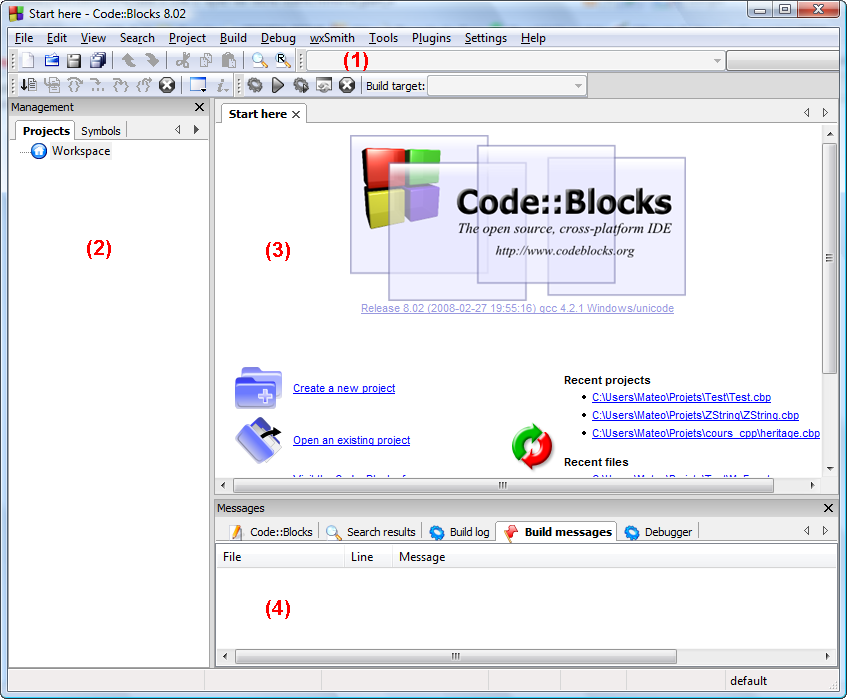
\includegraphics[width=\textwidth]{Chapter_I-2_CodeBlocks}
\end{figure}

نميّز أربعة أقسام رئيسية في واجهة البرنامج، و هي مرقّمة في الصورة :

\begin{enumerate}
  \item شريط الأدوات
(\textenglish{Toolbar}) :
يحتوي على كثير من الأزرار و لكنّنا سوف نستخدم بعضها فقط باستمرار، سأعود للحديث عن هذا فيما بعد.
  \item قائمة ملفات المشروع : توجد بيسار النافذة، تحتوي على كلّ الملفات المصدريّة المتعلقة بالبرنامج الذي تعمل عليه. تكون فارغة في البداية لأننا لم ننشئ أي ملف لحد الآن. سوف نبدأ بملأها خلال خمس دقائق من الآن بتقدّمك في هذا الفصل.
  \item المنطقة الرئيسية : هنا المساحة التي تكتب فيها الشفرة المصدرية الخاصة ببرنامجك بلغة الـ\textenglish{C}.
  \item منطقة الإشعار : و يدعوها البعض "منطقة الموت"، هنا تُعْرَضُ أخطاء الترجمة إذا كانت شفرة البرنامج تحوي خطأً ما. هذا الشيء يحدث كثيرا !
\end{enumerate}

ما يهمّنا الآن هو قسم محدد من شريط الأدوات. تجد فيه الأزرار التالية (بهذا الترتيب) :
\InlineCode{Compile}،
\InlineCode{Execute}،
\InlineCode{Compile \& Execute}،
\InlineCode{Recompile everything}
تذكّرهم جيّدا لأننا سنستخدمهم بانتظام.

\begin{figure}[H]
	\centering
	
\includegraphics{Chapter_I-2_Compile-toolbar}
\end{figure}

و هذا شرح عمل كلّ واحد من هذه الأزرار :

\begin{itemize}
  \item \textbf{\textenglish{Compile}} :
كل ملفّات الشفرة المصدرية الّتي كتبتها يتم ارسالها إلى المترجم الّذي يقوم بإنشاء الملف التنفيذي في حالة عدم وجود أخطاء. أمّا في حالة العثور على أخطاء (و هذا سيحدث عاجلا أم آجلا~!) فلن يتمّ إنشاؤه بل يعرض رسائل خطأ في منطقة الإشعار.
  \item \textbf{\textenglish{Execute}} :
يقوم بتشغيل آخر ملف تنفيذي تمّت ترجمته. يعني أنك ستستخدم هذا الزر لاختبار برامجك الّتي أنشأتها. طبعا يجب عليك ترجمة البرنامج قبل تشغيله. يمكننا أيضا استخدام الزرّ الثالث.
  \item \textbf{\textenglish{Compile \& Execute}} :
لا يجب أن تكون عبقريا لكي تعرف أنّه ليس إلا مجموع الزرّين السابقين. في الواقع هذا هو الزرّ الّذي ستستخدمه أكثر. في حالة ما إذا حدثت أخطاء في الترجمة لن يتمّ تشغيل البرنامج بل ستُعرض قائمة جميلة من الأخطاء التي يجب عليك تصحيحها أوّلا !
  \item \textbf{\textenglish{Recompile everything}} :
 عندما نستخدم
\textbf{\textenglish{Compile}}
يقوم
\textenglish{Code::Blocks}
في الحقيقة بترجمة الملفات الّتي عدّلتها فقط. أحيانا -فقط أحيانا- قد تحتاج إلى إعادة ترجمة جميع الملفّات. سنتحدّث لاحقا عن فائدة هذا الزر و أيضا عن كيفية عمل الترجمة بمزيد من التفصيل. حاليا لكي لا تختلط الأمور عليك يمكنك أن تعتبر أنّه غير مهمّ.
\end{itemize}

\begin{information}
أنصحك باستخدام اختصارات لوحة المفاتيح بدلا من الضغط على الأزرار، لأنّه شيء نكرّره كثيرا. تذكّر خصوصا أنّه يمكنك الضغط على
\InlineCode{F9}
بدل الزر
\InlineCode{Compile \& Execute}.
\end{information}

\subsection{إنشاء مشروع جديد}

لإنشاء مشروع جديد إذهب إلى قائمة
\InlineCode{File}
ثمّ
\InlineCode{New}
ثمّ
\InlineCode{Project}.
من النافذة الّتي تظهر اختر
\InlineCode{Console application}.

\begin{figure}[H]
	\centering
	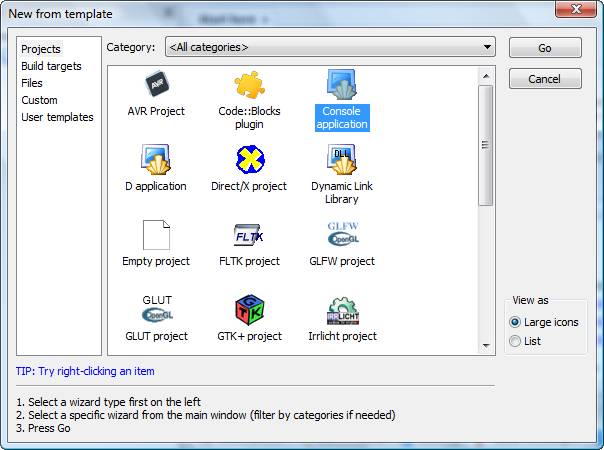
\includegraphics[width=0.8\textwidth]{Chapter_I-2_CodeBlocks-New-project}
\end{figure}

\begin{information}
كما تَرَى،
\textenglish{Code::Blocks}
يقترح عليك إنشاء عدد معتبر من أنواع البرامج الّتي تستخدم مكتبات
(\textenglish{Libraries})
معروفة مثل
\textenglish{SDL}
للـ\textenglish{2D}
و
\textenglish{OpenGL}
للـ\textenglish{3D}
و
\textenglish{Qt}
و
\textenglish{wxWidgets}
لإنشاء النوافذ الرسوميّة. حاليّا، هذه الأيقونات ليست سوى للزينة لأنّ المكتبات السابقة غير مثبّتة على حاسوبك لهذا لا يمكنك أن تجعلها تعمل. سوف نعود لهذه الأنواع الأخرى لاحقا. في هذه الأثناء لا يمكننا سوى أن نستخدم الـ\textenglish{Console}
لأنّك لا تملك بعد المستوى اللازم لانشاء أنواع أخرى من البرامج.
\end{information}

أنقر على
\InlineCode{Go}
لانشاء المشروع الجديد. ثم أنقر على
\InlineCode{Next}
فالصفحة الأولى ليس مهمّة. بعدها سيأتيك اختيار بين لغتي الـ\textenglish{C}
أو الـ\textenglish{C++}،
اختر الـ\textenglish{C}.

\begin{figure}[H]
	\centering
	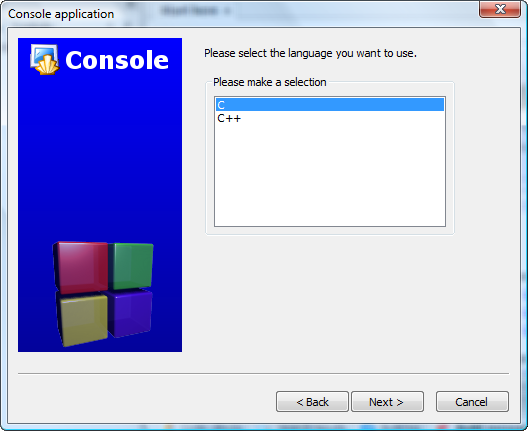
\includegraphics[width=0.8\textwidth]{Chapter_I-2_CodeBlocks-C}
\end{figure}

سيُطْلَبُ منك الآن إدخال اسم المشروع، و كذلك مسار المجلّد الذي تختاره لحفظ الملفّات فيه.

\begin{figure}[H]
	\centering
	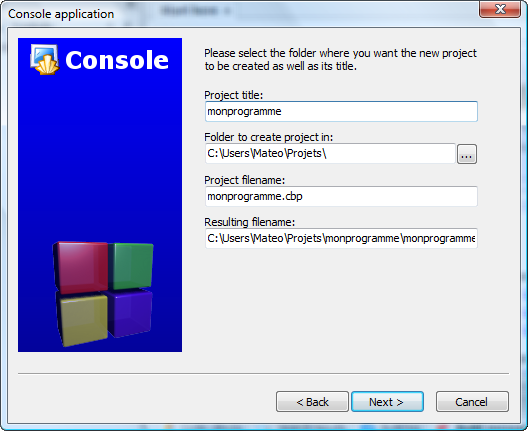
\includegraphics[width=0.8\textwidth]{Chapter_I-2_CodeBlocks_project-path}
\end{figure}

آخر خطوة تُطلب منك هي ، كيف ينبغي أن يترجم البرنامج، يمكنك ترك الخيارات على حالها، لن يكون لهذا أي تأثير على ما سنقوم به الآن (تأكّد أن إحدى الخانتين
"\textenglish{Release}"
أو
"\textenglish{Debug}"
تكون محدّدة على الأقل).

\begin{figure}[H]
	\centering
	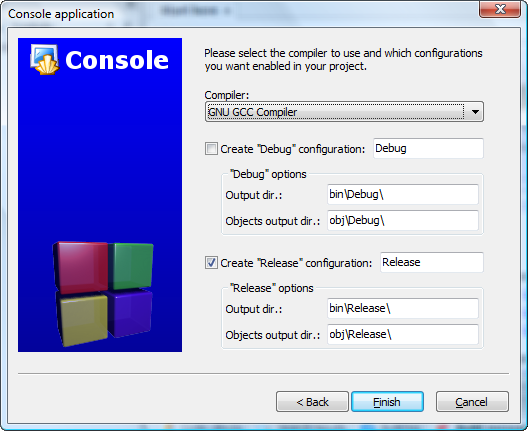
\includegraphics[width=0.8\textwidth]{Chapter_I-2_CodeBlocks_Compiler}
\end{figure}

إضغط على
\InlineCode{Finish}،
إنتهى !\\
لقد قام
\textenglish{Code::Blocks}
بإنشاء المشروع الأوّل و ملئه ببعض الشفرة المصدرية.

في الخانة الخاصة بالمشاريع على اليسار، قم بتوسيعها بالضغط على
'\InlineCode{+}'
لكي تظهر قائمة الملفات في المشروع. سيكون لديك على الأقل ملف يسمّى
\InlineCode{main.c}.
هذا هو كلّ شيء !

\section{\textenglish{Visual C++} (\textenglish{Windows} فقط)}

بعض التذكيرات حول
\textenglish{Visual C++} :

\begin{itemize}
  \item إنها البيئة التطويرية الخاصة بـ\textenglish{Microsoft}.
  \item برنامج مدفوع في الأصل، لكن توجد نسخة مجّانية منه تسمّى \textenglish{Visual C++ Express}.
  \item تمكّن من البرمجة باستخدام كلتا اللغتين
\textenglish{C}
و
\textenglish{C++}
(و ليس فقط
\textenglish{C++}
كما يوحي الاسم).
\end{itemize}

طبعا ستقوم بتحميل النسخة المجانية
\textenglish{Visual C++ Express}
(احذر، هو غير متوافق مع
\textenglish{Windows 7}
إلّا بداية من النسخة 2010) :

\begin{figure}[H]
	\centering
	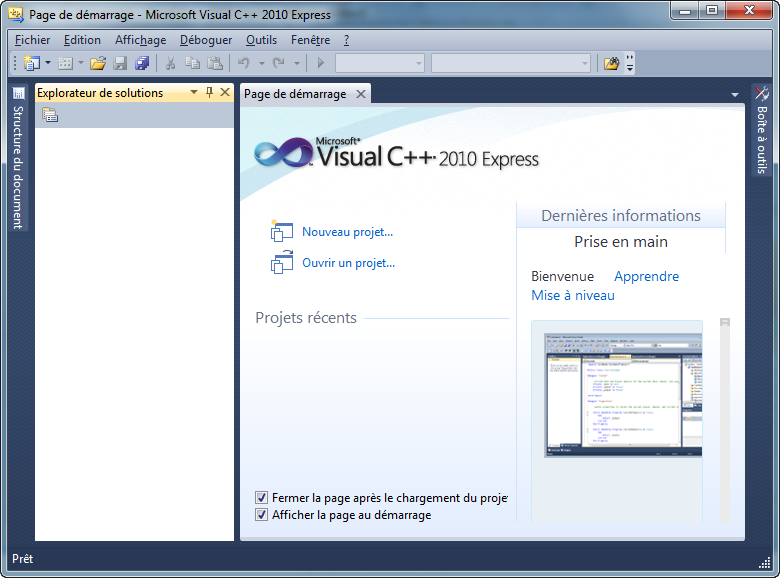
\includegraphics[width=\textwidth]{Chapter_I-2_Visual-Cpp}
\end{figure}

\begin{question}
ما الفرق بين هذه النسخة و النسخة "الحقيقيّة" ؟
\end{question}

لا تحتوي على محرّر موارد يسمح لك برسم الصور، الأيقونات أو النوافذ. هذا لا يهمّنا لأنّنا لن نحتاج إلى هذه الوظائف في هذا الكتاب. وجود هذه الوظائف أمر مستحسن لكنّه ليس لازما.

للتنزيل، زر موقع
\textenglish{Visual C++}.

\url{https://msdn.microsoft.com/fr-fr/express/aa975050.aspx}

و اختر تنزيل
\textenglish{Community 2015}
و اختر لغتك المفضّلة.

\subsection{التثبيت}

التثبيت سهل. سوف يقوم البرنامج بتحميل آخر نسخة من الأنترنت تلقائيا.\\
أنصحك بترك الخيارات كما هي.

بعد ذلك سيطلب منك التسجيل في غضون 30 يوما. لا تقلق، إنه سريع و مجاني لكن يجب القيام بذلك.

اضغط على الرابط المُعطى لك، ستدخل موقع
\textenglish{Microsoft}.
سجّل دخولك باستخدام
\textenglish{Windows Live ID}
(المكافئ لحساب
\textenglish{Hotmail}
أو
\textenglish{MSN})
أو قم بإنشاء واحد إذا لم يكن لديك، ثم أجب بعد ذلك على الأسئلة.

سيتم إعطاؤك في النهاية مفتاح تفعيل. انسخ هذا المفتاح في القائمة
\InlineCode{?}
ثم
"تسجيل المنتج".

\subsection{إنشاء مشروع جديد}

لإنشاء مشروع جديد، إذهب إلى قائمة
"ملف"
(\InlineCode{File})
ثمّ
"جديد"
(\InlineCode{New})
ثم
"مشروع"
(\InlineCode{Project}).
اختر
\InlineCode{Win32}
في العمود الأيسر ثمّ
\InlineCode{Win32 Console Application}.
ثمّ أدْخِل اسم مشروعك.

\begin{figure}[H]
	\centering
	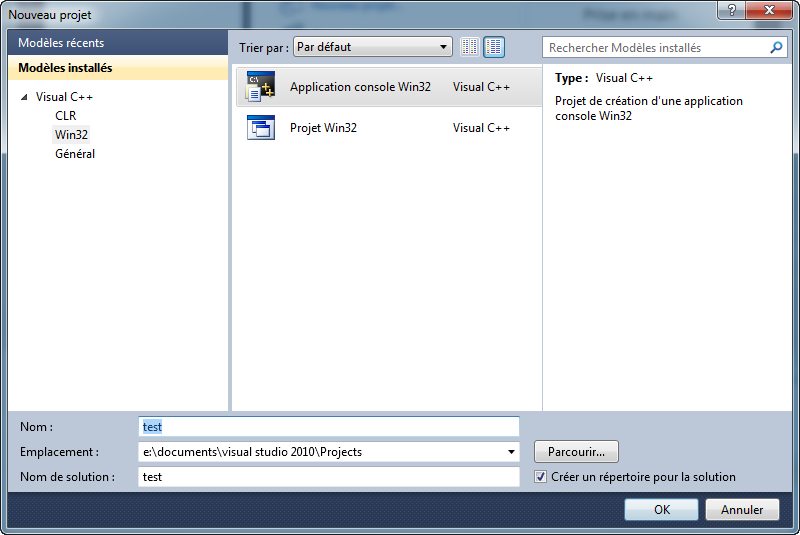
\includegraphics[width=0.8\textwidth]{Chapter_I-2_Visual-Cpp-New-project}
\end{figure}

وافق، ستظهر لك نافذة جديدة.

\begin{figure}[H]
	\centering
	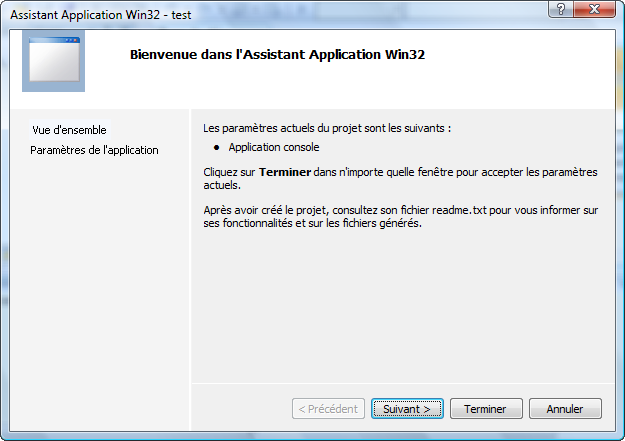
\includegraphics[width=0.8\textwidth]{Chapter_I-2_Visual-Cpp-Welcome}
\end{figure}

هذه النافذة لا تحوي أيّ شيء مهمّ، تابع فقط.

\begin{figure}[H]
	\centering
	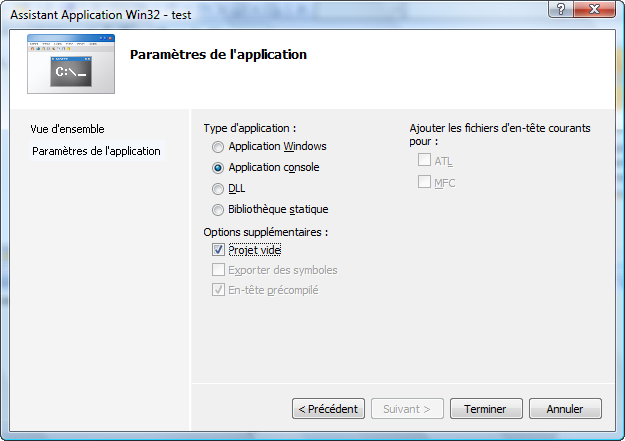
\includegraphics[width=0.8\textwidth]{Chapter_I-2_Visual-Cpp-Parameters}
\end{figure}

اختر
\InlineCode{Console application}
و تأكّد من إنشاء مشروع فارغ عن طريق تحديد
\InlineCode{Empty project}،
ثم اضغط على
"إنهاء"
(\InlineCode{Finish}).

\subsection{إضافة ملف مصدري جديد}

مشروعك فارغ لحدّ الآن. لإضافة ملف مصدري، اضغط باليمين على
"الملفات المصدرية"
(\InlineCode{Source files})
الموجود على اليسار، ثمّ اختر
"إضافة"
(\InlineCode{Add})
ثمّ
"عنصر جديد"
(\InlineCode{New element}).

\begin{figure}[H]
	\centering
	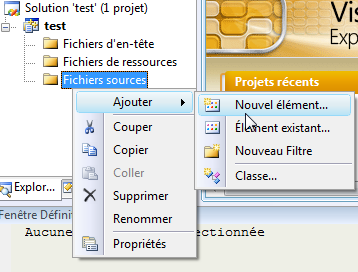
\includegraphics[width=0.5\textwidth]{Chapter_I-2_Visual-Cpp-New-source}
\end{figure}

اختر
\InlineCode{Visual C++}
على اليسار ثمّ
\InlineCode{C++ File}
(أعلمُ أنّنا لا ندرس
\textenglish{C++}
و لكن ليس لهذا أهميّة هنا). أدْخِل اسم الملف :
\InlineCode{main.c}

\begin{figure}[H]
	\centering
	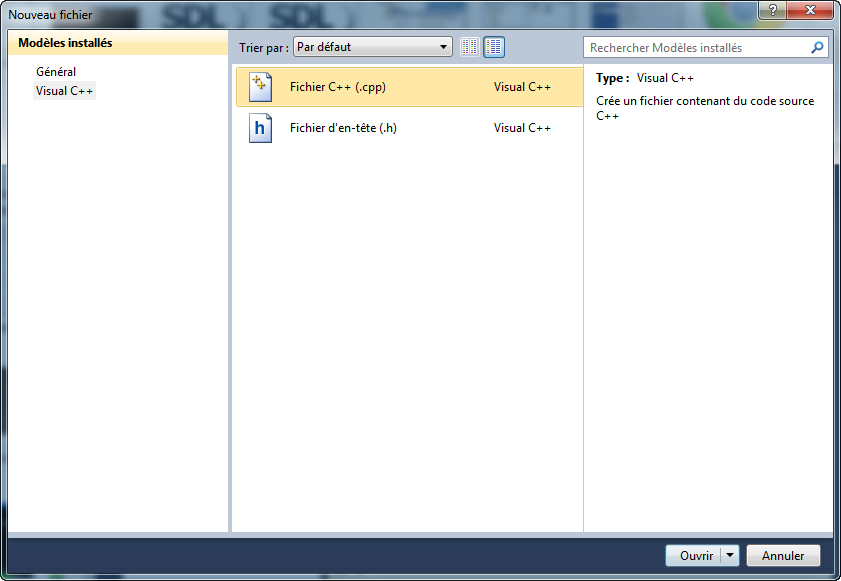
\includegraphics[width=0.8\textwidth]{Chapter_I-2_Visual-Cpp-New-file}
\end{figure}


ثم اضغط على
"إضافة"
(\InlineCode{Add}).
سيتم إنشاء ملفّ فارغ. أنصحك بحفظه بسرعة باسم
\InlineCode{main.c}.

انتهى، يمكنك الآن أن تبدأ في كتابة الشفرة.

\subsection{النافذة الرئيسيّة}

لنرى ما هي أهمّ أقسام النافذة الرئيسيّة في
\textenglish{Visual C++ Express}.

\begin{figure}[H]
	\centering
	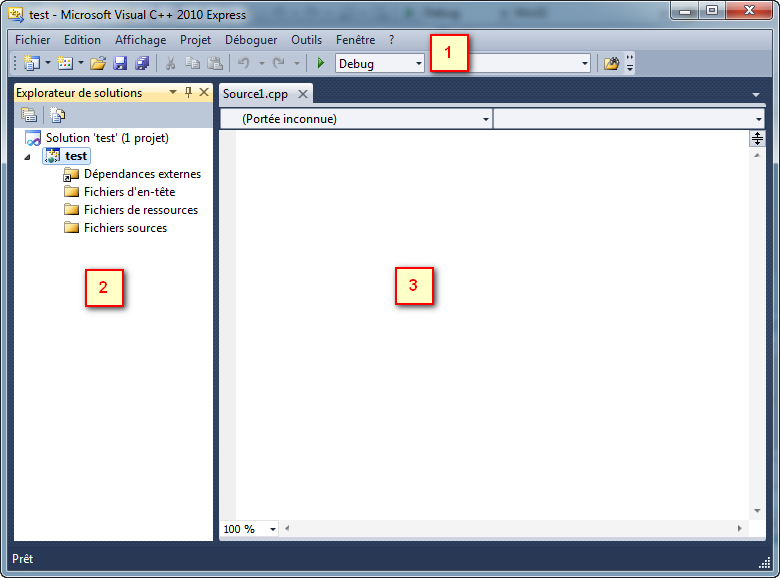
\includegraphics[width=\textwidth]{Chapter_I-2_Visual-Cpp-main}
\end{figure}

هذه النافذة تشبه مثيلتها في
\textenglish{Code::Blocks}.
و لكن رغم ذلك سوف نعيد رؤية معنى كلّ جزء.

\begin{enumerate}
  \item شريط الأدوات : فيه أزرار اعتيادية. لكن كما ترى لا يوجد أيّ زرّ للترجمة. يمكنك إضافته عن طريق النقر باليمين على هذا الشريط و اختيار
"تنقيح"
(\InlineCode{Debug})
و
"توليد"
(\InlineCode{Generate})
من القائمة.

كلّ هذه الأزرار لديها ما يكافئها في القوائم
\InlineCode{Debug}
و
\InlineCode{Generate}.
استخدام
\InlineCode{Generate}
ينشئ الملف التنفيذي (أي أنها تعني الترجمة). إذا استخدمت
\InlineCode{Debug / Execute}
فسوف يقترح عليك الترجمة قبل التشغيل. إختصارات لوحة المفاتيح :
\InlineCode{F7}
لتوليد المشروع و
\InlineCode{F5}
لتشغيله.
  \item هذه المساحة جدّ مهمّة، إذ أنها تحتوي على الملفات الخاصة بمشروعك. أنقر على
"مستكشف الحلول"
(\InlineCode{Solution explorer})
في الأسفل إن لم يكن فُعِل من قبل. سوف ترى أنّه قد تمّ إنشاء مجلّدات لفصل أنواع الملفّات المختلفة (مصدريّة، رأسيّة و موارد). سنتعرف لاحقا على مختلف أنواع الملفات التي تكوّن المشروع.
  \item المساحة الرئيسية : التي نعدّل فيها الملفّات المصدريّة.
\end{enumerate}

أكملنا جولتنا في
\textenglish{Visual C++}.
يمكنك إلقاء نظرة على
الخيارات
إن أردت لكن لا تأخذ من وقتك ثلاث ساعات هناك ! لأنه يوجد كثير منها.

\section{\textenglish{Xcode} (\textenglish{Mac OS X} فقط)}

هناك الكثير من البيئات التطويرية المتوافقة مع
\textenglish{Mac}
على غرار
\textenglish{Code::Blocks}
طبعا.\\
سأقدم لك البيئة الأكثر شهرة في الماك و هي
\textenglish{Xcode}.

\subsection{\textenglish{Xcode}،
 أين أنت ؟}

أغلب مستخدمي
\textenglish{Mac OS X}
ليسوا مبرمجين. لقد فهمت
\textenglish{Apple}
هذا، لذلك لم تثبّته افتراضيا مع النظام.\\
لحسن الحظ، لكلّ من يريد أن يبرمج، كلّ شيء جاهز.
\textenglish{Xcode}
متوفّر على
\textenglish{MacAppStore}.
ابدأ بأخذه من هناك.

أنصحك أيضا بإلقاء نظرة على الموقع الخاص بالمطوّرين لـ\textenglish{Apple}.

\url{https://developer.apple.com/}

سوف تجد هناك كمّا هائلا من من المعلومات المهمّة للتطوير على
\textenglish{Mac}.
يمكنك منه تحميل العديد من البرامج للتطوير.\\
لا تتردّد في التسجيل في
\textenglish{ADC} (\textenglish{Apple Development Connection})،
إنه مجاني و يساعدك على تتبع كل ما هو جديد.

\subsection{تشغيل \textenglish{Xcode}}

أوّل شيء يمكننا فعله هو إنشاء مشروع جديد، فلنبدأ بهذا. إذهب إلى
"ملف "
(\InlineCode{File})
ثمّ
"مشروع جديد"
(\InlineCode{New Project}).
ستفتح لك نافذة اختيار المشروع.

\begin{figure}[H]
	\centering
	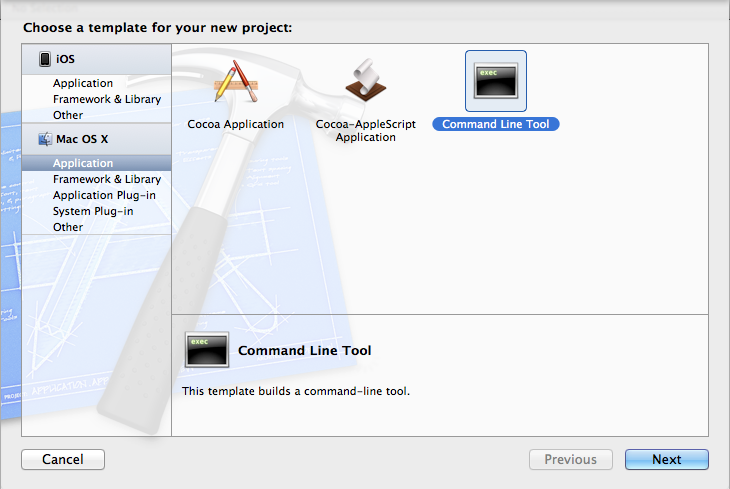
\includegraphics[width=0.8\textwidth]{Chapter_I-2_Xcode-New-project}
\end{figure}

اختر
\InlineCode{Application}
من اليسار ثمّ
\InlineCode{Command Line Tool}.
اضغط بعدها على
\InlineCode{Next}.
سوف يُطلب منكم بعدها حفظ مشروعك (كلّ مشروع يجب أن يحفظ منذ البداية) و اسمه. ضعه في المجلّد الّذي تريد.

بمجرّد إنشائه، سيتّم عرض مشروعك على شكل مجلّد يحتوي على العديد من الملفّات في الـ\InlineCode{Finder}.
الملف الّذي يملك الامتداد
\InlineCode{.xcodeproj}
يوافق ملف المشروع. إنه الملف الذي عليك اختياره في المرة القادمة لفتح مشروعك.

\subsection{نافذة التطوير}

في
\textenglish{Xcode}،
عندما تختار
\InlineCode{main.c}
تظهر لك نافذة شبيهة بهذه :

\begin{figure}[H]
	\centering
	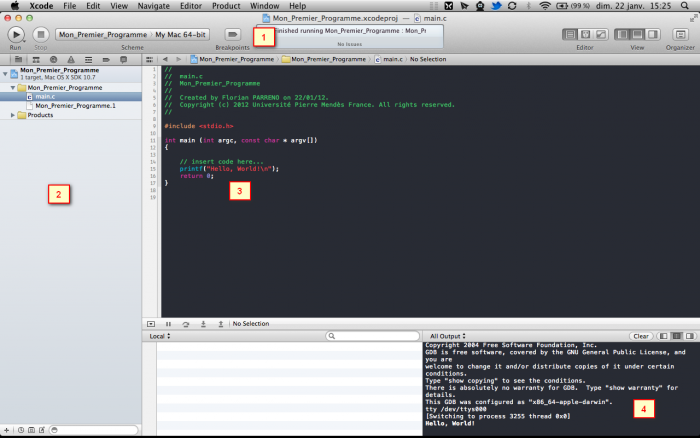
\includegraphics[width=\textwidth]{Chapter_I-2_Xcode-main}
\end{figure}

الواجهة مقسمة إلى أربعة أقسام، مرقمة هنا من 1 إلى 4 :

\begin{enumerate}
  \item الجزء الأوّل هو شريط الأزرار في الأعلى. أهمّ زرّ فيه هو
"تشغيل"
(\InlineCode{Run})
وظيفته تشغيل البرنامج.
  \item الجزء اليسار مخصص للتمثيل الشُجيري لمشروعك الخاص. بعض الأقسام تحتوي على الأخطاء، التحذيرات، إلخ. يقوم
\InlineCode{Xcode}
تلقائيّا بنقلك إلى القسم المهم. و هو الذي يحمل اسم المشروع.
  \item الجزء الثالث تتغيّر وظيفته حسب ما قمت بتحديده في الجزء الأيسر. و هنا يعرض محتوى الملف
\InlineCode{main.c}.
  \item أخيرا، الجزء الرابع يُظهر نتائج تشغيل البرنامج على الشاشة عندما تقوم بتشغيل البرنامج.
\end{enumerate}

\subsection{إضافة ملفّ جديد}

في البداية، لن تملك سوى ملف مصدري واحد و هو
\InlineCode{main.c}،
و لكن لاحقا عندما نتقدم في الدروس سأطلب منك إنشاء ملفات مصدريّة بنفسك، عندما تصبح برامجنا أكبر.

لإنشاء ملفّ جديد، اذهب إلى قائمة
\InlineCode{File}
ثمّ
\InlineCode{New File}.
سيطلب منك إدخال نوع الملف الذي تريد إنشاءه. توجّه إلى قائمة
\InlineCode{Mac OS X}
و اختر
\InlineCode{C and C++}
ثمّ
\InlineCode{C File}.
لاحظ هذه الصورة.

\begin{figure}[H]
	\centering
	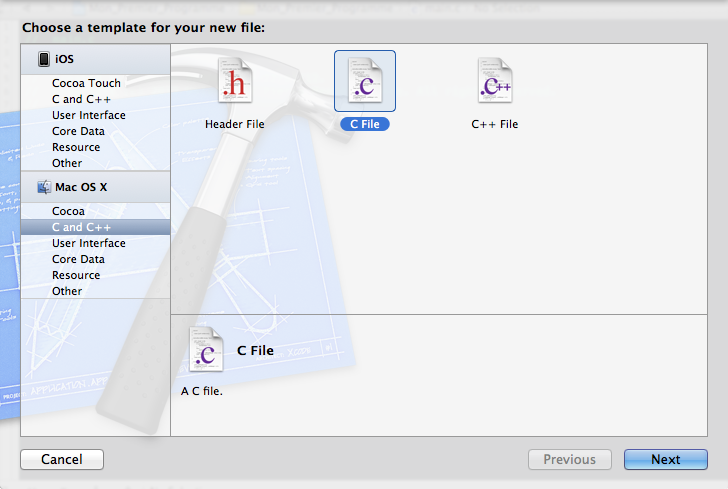
\includegraphics[width=0.8\textwidth]{Chapter_I-2_Xcode-C}
\end{figure}

يجب عليك إعطاء اسم لملفّك الجديد. امتداده يجب أن يبقى
\InlineCode{.c}.
أحيانا -كما سنرى لاحقا- يجب عليك أيضا إنشاء ملفّات بامتداد
\InlineCode{.h}.
الخانة
\InlineCode{Also create file.h}
مخصّصة لهذا الغرض. حاليّا هذا الخيار لا يهمّنا.

انقر بعدها على
\InlineCode{Finish}.
انتهى ! أصبح في مشروعك ملفٌ آخر غير الملف
\InlineCode{main.c}،
هنيئا لك فقد أصبحت الآن جاهزاً للبرمجة على الـ\InlineCode{Mac}.

\section*{ملخّص}

\begin{itemize}
  \item المبرمجون يحتاجون إلى ثلاثة أدوات : محرّر نصوص، مترجم و منقّح.
  \item من الممكن تثبيت هذه الأدوات منفصلة، لكنّه من المعتاد البوم الحصول على حُزمةٍ ثلاثة-في-واحد نسميها بيئة التطوير المتكاملة.
  \item \textenglish{Code::Blocks}،
\textenglish{Visual C++}،
و
\textenglish{Xcode}
تعدّ من بين بيئات التطوير الأكثر شهرة.
\end{itemize}
